% "{'chapitre':'slci_multiphy','classe':('PSI'),'type':('application'),'titre':'Mise à l\\'eau d\\'un robot sous-marin','source':'Concours Centrale - MP 2019','comp':['B2-02',],'corrige':True}"

\setchapterimage{fig_00.jpg}
\chapter*{Application \arabic{cptApplication} \\ 
Mise à l'eau d'un robot sous-marin -- \ifprof Corrigé \else Sujet \fi}
\addcontentsline{toc}{section}{Application \arabic{cptApplication} : Mise à l'eau d'un robot sous-marin  -- \ifprof Corrigé \else Sujet \fi}

\iflivret \stepcounter{cptApplication} \else
\ifprof  \stepcounter{cptApplication} \else \fi
\fi

\setcounter{question}{0}
\marginnote{Concours Centrale -- MP 2019}
\marginnote{\UPSTIcompetence[2]{B2-02}}
\begin{marginfigure}
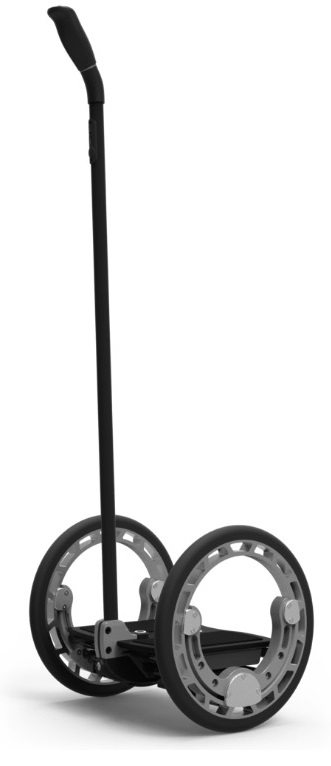
\includegraphics[width=\linewidth]{fig_01}
\end{marginfigure}



\ifprof
\else
Pour réaliser l’ensouillage sous-marin de câbles, ceux-ci sont déposés sur le fond marin par un navire câblier. Le robot sous-marin ROV (Remotely Operated Vehicle) est déposé sur le fond marin par un bateau support et ensouille le câble provenant
du navire câblier après l’avoir détecté et s’être aligné dans l’axe de celui-ci.

Pour transférer le ROV du pont du bateau support jusqu’à l’aplomb de la surface d’immersion une grue portique est utilisée. 
La grue portique est actionnée par un ensemble de deux vérins hydrauliques modélisés en un seul vérin équivalent pour cette étude.

Lors de la descente du ROV dans la mer, il est suspendu à un câble ombilical. Un bon équilibrage hydrostatique est
nécessaire pour assurer l’horizontalité du ROV pendant la descente.

\begin{marginfigure}
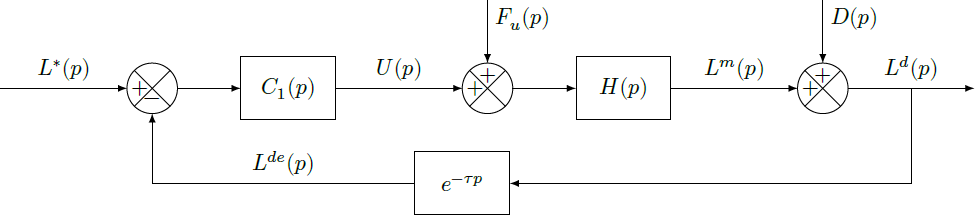
\includegraphics[width=\linewidth]{fig_03}
\end{marginfigure}

\begin{center}
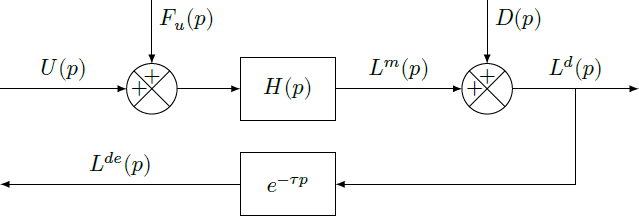
\includegraphics[width=\linewidth]{fig_02}
\end{center}

\fi

\begin{question}
À partir des figures précédentes, relier les composants du modèle de simulation
multiphysique de la grue portique. Quel(s) ensemble(s) n’ont pas été modélisés ?
\end{question}

\ifprof
\begin{corrige}~\\

\begin{center}
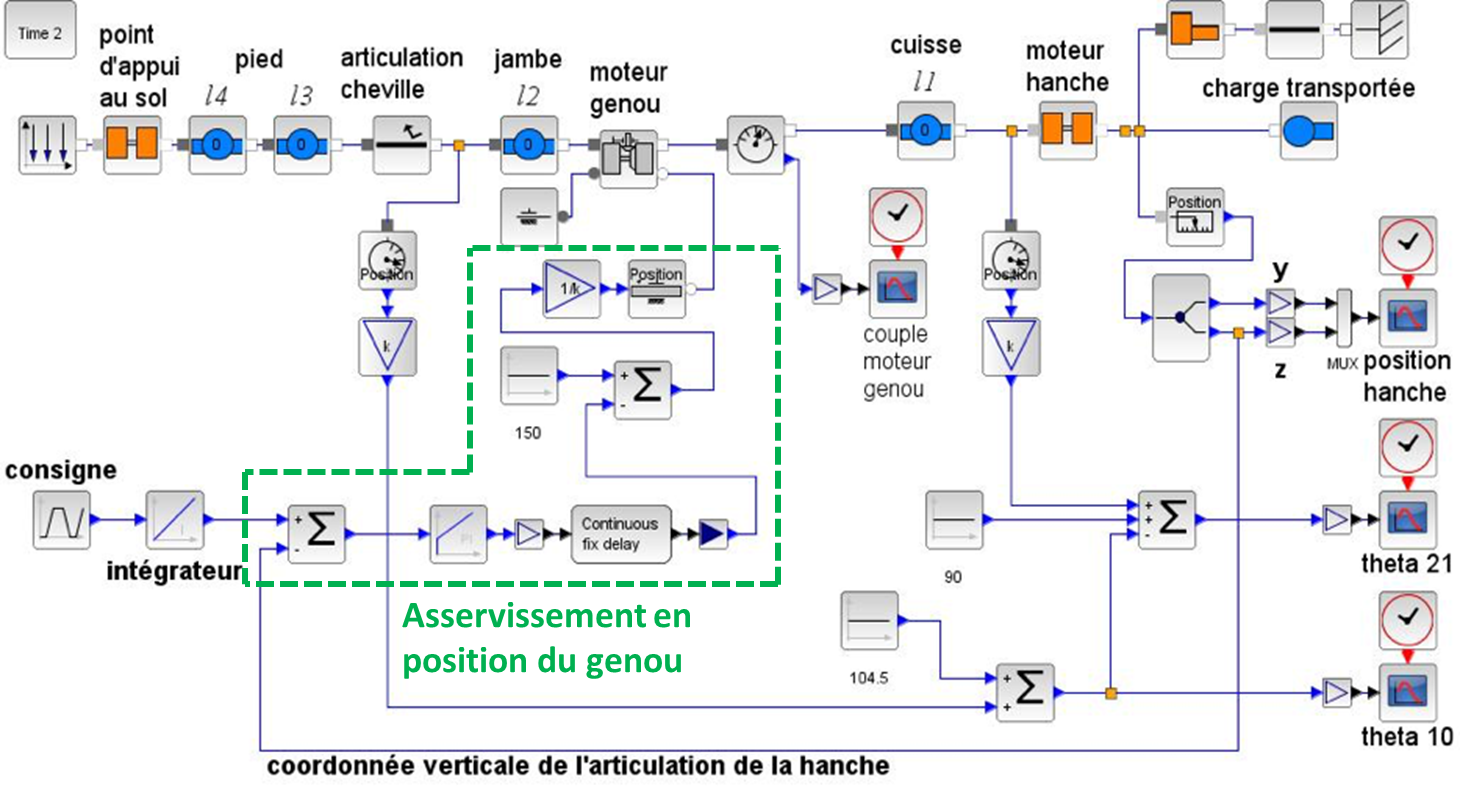
\includegraphics[width=\linewidth]{cor_01}
\end{center}
\end{corrige}
\else
\fi


\ifprof
\else
\begin{center}
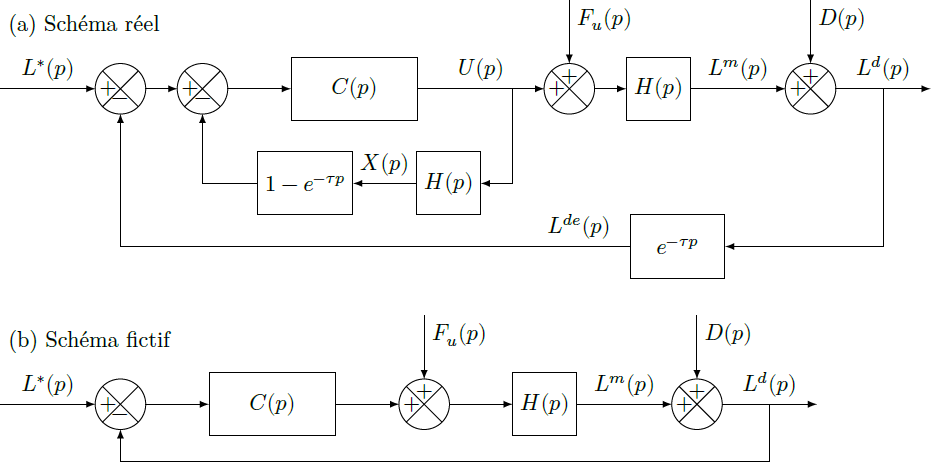
\includegraphics[width=.8\linewidth]{fig_04}
\end{center}
\fi

\ifprof
\else
\begin{marginfigure}
\centering

\includegraphics[width=3cm]{Cy_01_Ch_01_Application_01_qr}
\end{marginfigure}
\fi
